\documentclass{tufte-handout}
\usepackage{amsmath}

% Set up the images/graphics package
\usepackage{graphicx}
\setkeys{Gin}{width=\linewidth,totalheight=\textheight,keepaspectratio}
\graphicspath{{graphics/}}

\title{Syllabus: Introduction to Python}
\author{Chang Y. Chung}
\date{January 2014}

\usepackage{booktabs}
\usepackage{units}
\usepackage{fancyvrb}
\fvset{fontsize=\normalsize}
\usepackage{multicol}
\usepackage{listings}

\usepackage[activate={true,nocompatibility},final,tracking=true,kerning=true,spacing=true,factor=1100,stretch=10,shrink=10]{microtype}
\microtypecontext{spacing=nonfrench}

\usepackage{soul} % for strike through

\begin{document}
\maketitle

\begin{marginfigure}%
  
\includegraphics[width=\linewidth]{python}
  \caption{Python logo from \url{http://www.python.org}. The name is not
    after those dangerous reptiles; it is from the seventies comedy series
    ``Monte Python's Flying Circus''.}
  \label{fig:Python}
\end{marginfigure} 

\section{Introduction}\label{sec:introduction}
Python is a popular, general-purpose, multi-paradigm,
open-source, scripting language. It is designed to emphasize code
readability -- has a clean syntax with high level data types. It is
suited for interactive work and quick prototyping, while being powerful
enough to write large applications in.

Python has a large number of available and well-written modules for
everything from abstract syntax trees to ZIP file manipulation. Its
ecosystem features an extensive set of tools including a JIT
compiler\footnote{PyPy (\url{http://pypy.org})} and fancy
IDE's\footnote{For instance, IPython (\url{http://ipython.org})}.

In this half-day workshop, you will be introduced to basic Python
language syntax and to its ecosystem.

\begin{marginfigure}%
  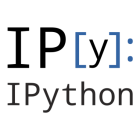
\includegraphics[width=0.4\linewidth]{ipython}
  \caption{IPython (\url{http://ipython.org}) is a rich architecture for
    interactive computing. Version 1.0.0 was released on Aug, 2013.}
  \label{fig:IPython}
\end{marginfigure} 

\begin{marginfigure}%
  
\includegraphics[width=0.4\linewidth]{numpy}
  \caption{NumPy (\url{http://www.numpy.org}) implements an N-dimensional
    array and is considered as the fundamental package for
    scientific computing with Python.}
  \label{fig:NumPy}
\end{marginfigure} 

\section{Objectives}\label{sec:objectives}
After taking this course, you should be able to:
\begin{itemize} \itemsep1pt \parskip0pt \parsep0pt
  \item use Python interactively
  \item execute a Python script at the shell prompt
  \item use Python types, expressions, and None
  \item use string literals and string type % raw and unicode strings as well?
  \item use Python statements (if...elif..else, for, pass, continue,
\ldots)
  \item understand the difference between expressions and statements
  \item understand assignment semantics
  \item write and call a simple function % (lexical scoping rule?)
  \item utilize high-level data types such as lists and dictionaries
  \item understand the difference between mutable and immutable types
  \item write a simple class and access methods and attributes
  \item import and utilize a module % (Beautiful Soup?)
  \item read from and write to a text file
  \item understand interpreter and compilers: CPython, PyPy, Cython
  \item see demonstration of IDE's: IDLE, IPython, IPython
     Notebook, hosted environments
  \item understand the role of package managers: easy\_install, pip
  \item understand what NumPy does and what SciPy is (are?) 
  \item learn about resources for learning Python\footnote{tutorials,
        books, MOOC's, videos, web sites, Python Koans,
        Python Challenge, and Project Euler}

\end{itemize}

\section{Intended Audience}\label{sec:intended_audience}
This workshop is for those who have some experience in using at least
one scripting language\footnote{Stata, R, MATLAB, Perl, Ruby, emacs
lisp, bash, or PowerShell, etc.} but who do not know Python. It is
assumed that you can edit a text file using your favorite editor, and be
able to execute your script file on the command line of a shell.

\section{Installation}\label{sec:installation}
Python comes pre-installed in Mac OS X and Linux. Since Python 3 is not
backward compatible and not all the modules are upgraded into Python 3,
we will use the latest version of Python 2 (2.7 as of writing this), 
which is the default for OS X and Linux.

A nice instruction for installing Python on Windows is at The
Hitchhiker's Guide to Python
site\footnote{\url{http://docs.python-guide.org/en/latest/starting/install/win/}}.

Installation of pip is optional but encouraged, since pip is the tool for
installing and managing Python packages. An installation guide is
at \url{http://www.pip-installer.org/en/latest/installing.html}.

\begin{figure*}[ht]
  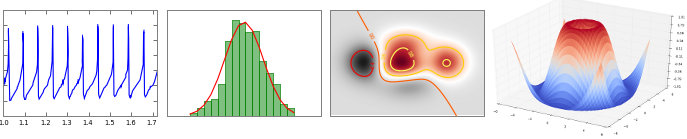
\includegraphics[width=0.8\linewidth]{matplotlib.png}%
  \caption{These plots are generated using the matplotlib module
    (\url{http://matplotlib.org}), which is a python 2D
    plotting library created by John Hunter, who unfortunately
    died of complications from cancer treatment in 2012.}%
  \label{fig:Matplotlib Plot Examples}%
\end{figure*}

\section{Location and Date}\label{sec:location_and_date}
% OPR Computer Lab: \#217 Wallace Hall (or TBA)
\noindent Location: \st{\#217 Wallace Hall}
   Bowl 001 Robertson Hall (Lower Level)

\noindent Date: Tue Jan. 14th, 2014  1:30 -- 4:30 pm

\section{Schedule}\label{sec:schedule}
\begin{table}[ht]
  \fontfamily{ppl}\selectfont
  \begin{tabular}{lll}
    \toprule
    Section & Format & Topic \\
    \midrule
    Basic Syntax & Lecture \& Quiz & Hello World to List \& Dict \\
    Intermediate Syntax & Lecture \& Quiz & Mutable to File IO \\
    Ecosystem & Demo \& QA & Compilers to Resources \\
    (Optional) & Survey & Evaluation \\
    \bottomrule
  \end{tabular}
  \caption{Each of the three sections will last 50 minutes total with a
    15-20 minute break in between the sections. At the end of each
    section, a homework or in-depth lab material will be provided.}
  \label{tab:Schedule}
\end{table}

\end{document} 

